\documentclass[nocrop, rm, english]{style/template}

% Options
%
% rm          - Roman font
% sf          - Sanserif font
% crop        - Crop marks (cross shaped) 17x24 cm (+3 mm for each side) centered on an A4
% nocrop      - Without crop marks, respeta el tama�o 17x24 cm 
%
% castellano  - For publications written in Spanish
% valencia    - For publications written in Valencian
% english     - For publications written in English

% ---------------------------------------------------------------------
% Custom settings

\usepackage[T1]{fontenc}

\ifcastellano\usepackage[spanish,es-tabla,es-sloppy]{babel}\fi
\ifvalencia\usepackage[catalan]{babel}\fi
\ifenglish\usepackage[english]{babel}\usepackage{csquotes}\fi
\newcommand{\sen}{\on{sen}}	

\usepackage{xcolor}
\usepackage{array,booktabs}
\usepackage{tabularx,longtable,multicol}
\usepackage{amssymb}
\usepackage{natbib}


\colorlet{colorEnlace}{black}

\usepackage[
	{colorlinks},
	{linkcolor=colorEnlace},
	{citecolor=colorEnlace},
	{urlcolor=colorEnlace},
	{bookmarksnumbered},
	{breaklinks},
	]{hyperref}

% ---------------------------------------------------------------------
% ---------------------------------------------------------------------
% International System Units

\usepackage{eurosym}
\usepackage{siunitx}

\ifenglish
	\sisetup{output-decimal-marker={.}}
\else
	\sisetup{output-decimal-marker={,}}
\fi

\DeclareSIUnit[number-unit-product = {\;}] \EURO{\geneuro}



% ---------------------------------------------------------------------

\newcommand{\ingles}[1]{\textit{#1}}

% ------------------------------------------------------------------------

\usepackage{xspace}

\newcommand{\angles}[1]{\textit{#1}\/}
\newcommand{\miUrl}[1]{{\small%
	{\underline{#1}}}}

\newcommand{\matlabr}{{\sc Matlab}$^\circledR$\xspace}
\newcommand{\simulinkr}{\textit{Simulink}$^\circledR$\xspace}
\newcommand{\matlab}{{\textsc{Matlab}}\xspace}
\newcommand{\simulink}{\textit{Simulink}\xspace}

\newcommand{\scr}{\textit{script\/}\xspace}
\newcommand{\scrs}{\textit{scripts\/}\xspace}

% ------------------------------------------------------------------------

\definecolor{griset}{rgb}{.925, .925, .925}


\newsavebox{\mybox}
\newenvironment{parrafoDestacado}
	{%
	\fboxsep = 2ex
	\fboxrule = .4pt
  	\begin{lrbox}{\mybox}%
  	\begin{minipage}{.85\textwidth-2\fboxsep}\itshape\parskip=2ex
	}
	{%
	\end{minipage}
  	\end{lrbox}%
	\begin{flushright}
		\colorbox{griset}{\usebox{\mybox}}%
	\end{flushright}
	}
	

% ------------------------------------------------------------------------
% Chapter abstract

\newsavebox{\myboxb}
\newenvironment{Resumen}
	{%
	\vspace*{-2.0cm}
	\fboxsep = 0pt
	\fboxrule = 0pt
  	\begin{lrbox}{\myboxb}%
  	\begin{minipage}{.85\textwidth}\itshape\parskip=2ex\parindent=2em
	}
	{%
	\end{minipage}
  	\end{lrbox}%
	\begin{flushright}
		\usebox{\myboxb}%
	\end{flushright}
	\vspace{0.5cm}
	}

% ---------------------------------------------------------------------
% ---------------------------------------------------------------------
% Math symbols

\newcommand{\on}{\operatorname}

% ---------------------------------------------------------------------
% ---------------------------------------------------------------------
% Theorems and examples

\ifcastellano
	\newtheorem{teorema}{\upshape\bfseries Teorema}[section]
	\newtheorem{lema}{\mdseries\scshape Lema}[section]
	\newtheorem{proposicion}{\upshape\bfseries Proposici�n}[section]
	\newtheorem{ejemplo}{\bfseries\scshape Ejemplo}[section]
\fi

\ifvalencia
	\newtheorem{teorema}{\upshape\bfseries Teorema}[section]
	\newtheorem{lema}{\mdseries\scshape Lema}[section]
	\newtheorem{proposicion}{\upshape\bfseries Proposici�}[section]
	\newtheorem{ejemplo}{\bfseries\scshape Exemple}[section]
\fi

\ifenglish
	\newtheorem{teorema}{\upshape\bfseries Theorem}[section]
	\newtheorem{lema}{\mdseries\scshape Lemma}[section]
	\newtheorem{proposicion}{\upshape\bfseries Proposition}[section]
	\newtheorem{ejemplo}{\bfseries\scshape Example}[section]
\fi

% ---------------------------------------------------------------------
% ---------------------------------------------------------------------

\newcommand{\FuenteEjemplos}{\small}

% ---------------------------------------------------------------------
% ---------------------------------------------------------------------
% Theorem and examples

\usepackage[most]{tcolorbox}


% ---------------------------------------------------------------------
% Ejemplo: custom environment for examples
\usepackage[nameinlink,capitalize]{cleveref}

\definecolor{colorFonsExemples}{rgb}{0.95,0.95,0.95}
\colorlet{colorFonsCapcaleraExemples}{black!18!white}

\newtcbtheorem[
	auto counter,
	number within = chapter,
	]{texemple}{\bfseries Example}{
		enhanced jigsaw,
		breakable,
		pad at break* = 1mm,
		arc = 0.0mm,
		%
		sharpish corners,
		leftrule = 0pt, rightrule = 0pt,
		bottomrule = 0pt, toprule = 0pt,
		%
		colback = colorFonsExemples,
		colframe = colorFonsExemples,
		description color = black,
		coltitle = black,
		colbacktitle = colorFonsCapcaleraExemples,
		fonttitle = \FuenteEjemplos,
		fontupper = \FuenteEjemplos,
		toptitle = 0.45ex, bottomtitle = 0.25ex,
		before skip = 4ex, after skip = 4ex,
		}{ejemplo}

\newcounter{ejemploCounter}[chapter]
\renewcommand{\theejemploCounter}{\thechapter.\arabic{ejemploCounter}}
\newenvironment{Ejemplo}[2]
	{
	\refstepcounter{ejemploCounter}
	\begin{texemple}{#1}{#2}
	\parskip = \separaParrafos 
	\parindent = \indentaParrafos 
	\abovedisplayshortskip = -1.0ex plus 0ex minus 0.25ex
	\belowdisplayshortskip = 2.0ex plus 1ex minus 0.0ex	
	\abovedisplayskip = -1.0ex plus 0ex minus 0.25ex
	\belowdisplayskip = 2.0ex plus 1ex minus 0.0ex
	}
	{
	\end{texemple}
	}
\Crefname{ejemploCounter}{Example}{Examples}


\newenvironment{enunciadoEjercicio}{\itshape}{} %\slshape

\newcommand{\finEjemplo}[1]{%
	\vspace{1ex}
	\begin{flushright}
		\slshape\FuenteEjemplos
		{Fin del ejemplo} \ref{ejemplo:#1}
		\hspace{1em}\textcolor{colorFonsCapcaleraExemples}{$\blacksquare$}
	\end{flushright}
	%
	\vspace{-1ex}
	}

		
% ---------------------------------------------------------------------
% Gray zone

\makeatletter
\newenvironment{zonaGrisa}{\begin{tcolorbox}[
		width = \textwidth-\@totalleftmargin,
		enhanced jigsaw,
		sharpish corners,
		breakable,
		boxrule=0pt,
		leftrule = 0pt, rightrule = 0pt,
		left=1em,right=1em,top=3ex,bottom=1ex, 
		bottomrule=0pt,toprule=0pt,
		colback=colorFonsSolucions,
		colframe=colorMarcSolucions,
		coltitle = black,
		fonttitle=\bfseries\upshape,
		fontupper = \SelectFont\selectfont,
		before skip = 0ex, after skip = 4ex,
		]\parskip = 2ex}{\end{tcolorbox}}
\makeatother		
\usepackage{titletoc}
\usepackage{lipsum}
\usepackage{multirow}

\usepackage{lipsum}

\usepackage{minitoc}
\setcounter{minitocdepth}{1}

\usepackage{fontspec}
\newfontfamily\ExampleFont[Mapping=tex-text]{QTCloisteredMonk}
\newfontfamily\TitleFont[Mapping=tex-text]{QTFlorencia}
\newfontfamily\QuotesFont[Mapping=tex-text]{IBMPlexSerif-Light}
\usepackage{unicode-math}
\setmathfont{Libertinus Math}

\usepackage{lettrine}
\usepackage{GoudyIn}

\usepackage{xcolor} 
\renewcommand{\LettrineFontHook}{\color{purple}\GoudyInfamily{}}
\LettrineTextFont{\itshape}
\setcounter{DefaultLines}{2}%

\definecolor{crown}{RGB}{0,51,0}
\definecolor{cross}{RGB}{102,102,0}
\definecolor{flower}{RGB}{76,0,153}
\definecolor{snor}{RGB}{102,0,204}
\definecolor{backcover}{RGB}{8,8,70}

\usepackage{xpatch}
\newlistof{equations}{equ}{List of Equations}
\newcommand{\myequations}[1]{%
	\csname phantomsection\endcsname % if hyperref is loaded
	\addcontentsline{equ}{equations}{\small\protect\numberline{\theequation} #1}%
}

\makeatletter
\xpretocmd{\@chapter}{\addtocontents{equ}{\protect\addvspace{10\p@}}}{}{}{}%
\makeatother

\newlistof{examples}{exam}{List of Examples}
\newcommand{\myexamples}[1]{%
	\csname phantomsection\endcsname % if hyperref is loaded
	\addcontentsline{exam}{examples}{\small\protect\numberline{\theejemploCounter} #1}%
}

\makeatletter
\xpretocmd{\@chapter}{\addtocontents{exam}{\protect\addvspace{10\p@}}}{}{}{}%
\makeatother

\usepackage{style/psvectorian}
\usepackage[]{pstricks}

\usepackage{upquote}
\usepackage{style/pgf-pie}
\usepackage{subcaption}

\usepackage{acro}
\acsetup{cite/cmd = {\citep}, make-links = true}

\DeclareAcronym{vip}{short = VIP, long  = very important paper, cite = vip}
\DeclareAcronym{phd}{short = PhD, long  = please hold the door}

\usepackage{soul}

\usepackage[toc]{appendix}

\usepackage{pgfplots}
\pgfplotsset{every tick label/.append style={font=\scriptsize}}

\newcommand{\revisions}[1]{{\leavevmode\color{magenta}#1}}

\usepackage{pdfpages}

\usepackage{tikz}
\makeatletter
\newcommand*{\radiobutton}{%
	\@ifstar{\@radiobutton0}{\@radiobutton1}%
}
\newcommand*{\@radiobutton}[1]{%
	\begin{tikzpicture}
	\pgfmathsetlengthmacro\radius{height("X")/2}
	\draw[radius=\radius] circle;
	\ifcase#1 \fill[radius=.6*\radius] circle;\fi
	\end{tikzpicture}%
}
\makeatother

\usetikzlibrary{shapes.geometric, arrows, positioning}
\tikzstyle{chapter} = [rectangle, text width=2cm, text centered, draw=black, fill=white]
\tikzstyle{arrow} = [thick,->,>=stealth]
\tikzstyle{line} = [thick]


\usepackage{etoolbox}
\preto\chapter\acresetall

\usepackage{pagecolor}

\usepackage{soul}
\makeatletter
\NewDocumentCommand{\sotwo}{O{red}O{black}+m}
{%
	\begingroup
	\setulcolor{#1}%
	\setul{-.5ex}{.4pt}%
	\def\SOUL@uleverysyllable{%
		\rlap{%
			\color{#2}\the\SOUL@syllable
			\SOUL@setkern\SOUL@charkern}%
		\SOUL@ulunderline{%
			\phantom{\the\SOUL@syllable}}%
	}%
	\ul{#3}%
	\endgroup
}
\makeatother

\makeatletter
\newcommand{\namerefname}[1]{\edef\@currentlabelname{#1}}% New \nameref name
\makeatother

% ---------------------------------------------------------------------
% Path for graphics

\graphicspath{
	{./fig/}
	{./logo/}
	}

% ---------------------------------------------------------------------

\newcommand{\department}{Science Fiction Department}

\title{
	On Writing your Ph.D. Dissertation \\[3ex]
	\mdseries \LARGE	Ph.D. Dissertation
	}

\author{
	\parbox{\textwidth}{\centering%
			Miguel Domingo\\[1ex]
			Supervised by Prof. Oak\\[.5ex]
		}
	}

\date{July 1969}

% ---------------------------------------------------------------------
% ---------------------------------------------------------------------
% ---------------------------------------------------------------------

\begin{document}
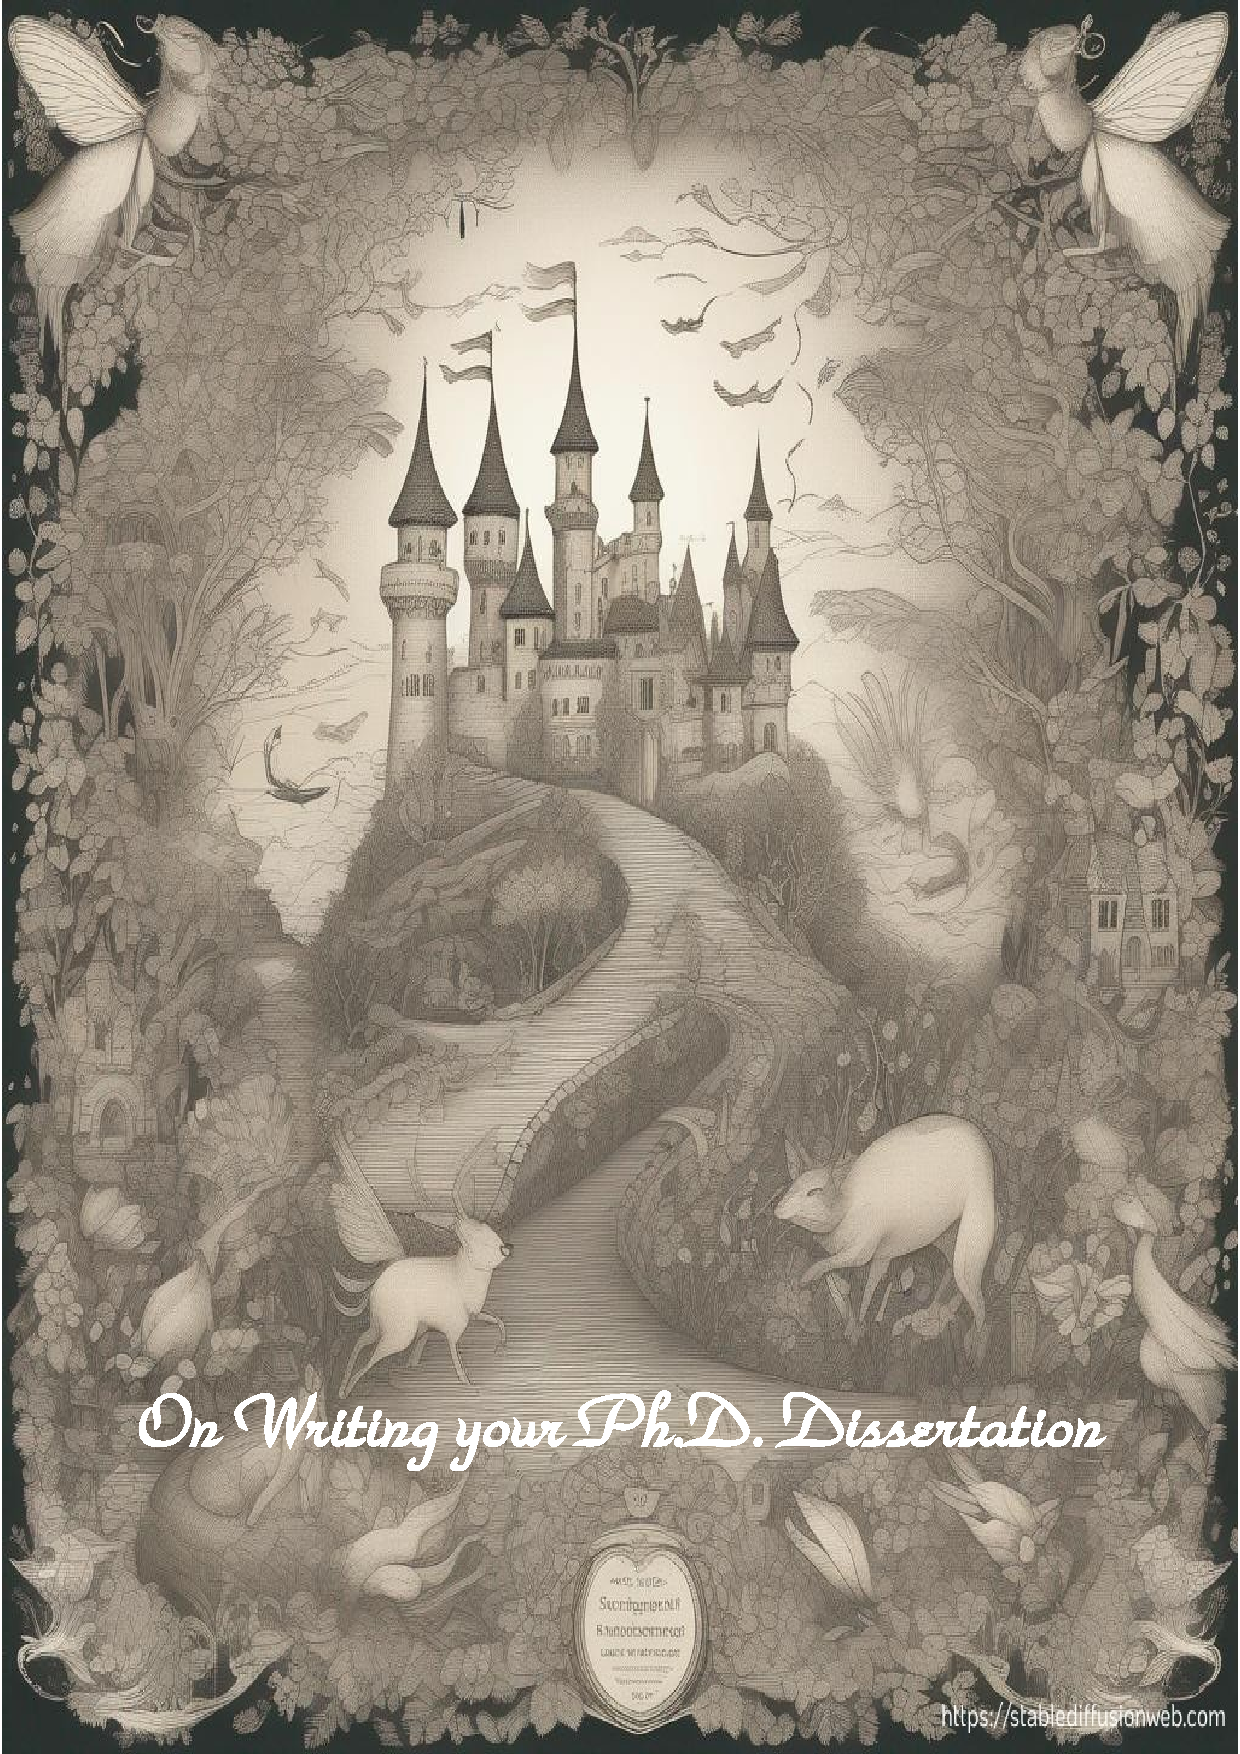
\includepdf{cover/frontcover.pdf}

\dominitoc

\frontmatter

\titlecontents{psection}[2.3em]
{} {\contentslabel{2.3em}} {} {\titlerule*[1pc]{.}\contentspage}
\titlecontents{psubsection}[5.5em]
{} {\contentslabel{3.2em}} {} {\titlerule*[1pc]{.}\contentspage}

% -------------------------------------------------------
% Title page

\maketitle



% -------------------------------------------------------

\cleardoublepage
\chapter*{Acknowledgments}
\rput[c](0.46\textwidth,6.5){\psvectorian[scale=0.5]{24}}

This is probably the most satisfactory chapter to write. It puts an end to a phase of your life, and allows you some time to remember all that has happened.

\begin{flushright}
	The Moon, July 21$^{\mathrm{th}}$ 1969.
\end{flushright}

\cleardoublepage
\chapter*{Abstract}\chaptermark{Abstract}
\rput[c](0.46\textwidth,6.5){\psvectorian[scale=0.5]{24}}

This document pretends to illustrate how to use this template for writing your dissertation.

\cleardoublepage
\chapter*{Preface}\chaptermark{Preface}\addcontentsline{toc}{chapter}{Preface}\mtcaddchapter
\rput[c](0.46\textwidth,6.5){\psvectorian[scale=0.5]{24}}

This is a good place to motivate the problems you are facing on your dissertation and the proposals you made to solve them.

\pagebreak

The scientific goals of this thesis are divided into two main groups:

\begin{enumerate}
	\item \textbf{Group 1}. We propose to do things.
	\item \textbf{Group 2}. We did things!
\end{enumerate}

This dissertation is structured in 7 chapters that relate as follows:

\newlength{\introlength}\settowidth{\introlength}{test \nameref{ch:example}}\setlength{\introlength}{0.6\introlength}

\begin{figure*}[!h]
	\centering
	\footnotesize
	\resizebox{\textwidth}{!}{
	\begin{tikzpicture}[node distance=0.75cm]
		%\scriptsize
		\node (intro) [chapter, text width=\the\introlength] {Ch. \ref{ch:example} \\ \nameref{ch:example}};
		\node (mt) [chapter, text width=\the\introlength, below=0.75cm of intro] {Ch. \ref{ch:example} \\ \nameref{ch:example}};
		\node (lmod) [chapter, text width=\the\introlength, below=0.75cm of mt] {Ch. \ref{ch:example} \\ \nameref{ch:example}};
		\node (imt) [chapter, text width=\the\introlength, left=0.5cm of lmod] {Ch. \ref{ch:example} \\ \nameref{ch:example}};
		\node (snor) [chapter, text width=\the\introlength, right=0.5cm of lmod] {Ch. \ref{ch:example} \\ \nameref{ch:example}};
		\node (imthd) [chapter, text width=\the\introlength, below=of lmod] {Ch. \ref{ch:example} \\ \nameref{ch:example}};
		\node (conclusions) [chapter, text width=\the\introlength, below=of imthd] {Ch. \ref{ch:example} \\ \nameref{ch:example}};
		\draw [arrow] (intro) -- (mt);
		\draw [arrow] (mt) -| (imt);
		\coordinate [above=0.5cm of lmod](lmodpoint);
		\coordinate [above=0.5cm of snor](snorpoint);
		\coordinate [left=1.5cm of snorpoint](intropoint);
		\draw [line] (intro) -| (intropoint);
		\draw [line] (mt) -| (intropoint);
		\draw [arrow] (lmodpoint) -- (lmod);
		\draw [arrow] (snorpoint) -- (snor);
		\draw [line] (lmodpoint) -- (snorpoint);
		\draw [arrow] (imt) |- (imthd);
		\draw [arrow] (lmod) -- (imthd);
		\draw [arrow] (snor) |- (imthd);
		\draw [arrow] (imthd) -- (conclusions);
	\end{tikzpicture}
	}	
\end{figure*}

The content of each chapter is:

\begin{description}
	\item[\cref{ch:example}] showcases the usage of this dissertation template, spiced with a pinch of humor.
\end{description}

These chapters are complemented by the following appendixes:

\begin{description}
	\item[\cref{ap:appendix}] showcases how an appendix looks like.
\end{description}
	
% -------------------------------------------------------
\cleardoublepage
\tableofcontents


\cleardoublepage
\chapter*{Acronyms}\chaptermark{Acronyms}\addcontentsline{toc}{chapter}{Acronyms}\mtcaddchapter
\rput[c](0.46\textwidth,6.5){\psvectorian[scale=0.5]{24}}

\printacronyms[heading=none]


% -------------------------------------------------------
% Arabic page numbers

\mainmatter

% -------------------------------------------------------
% -------------------------------------------------------
% -------------------------------------------------------
% Chapters

\cleardoublepage
\chapter{This Is a Fairly Long Title to Check How it Looks Like}
\label{ch:example}
\rput[r](0.585\textwidth,2.5){\psvectorian[color=cross,scale=0.4]{58}}
\begin{Resumen}
	\QuotesFont
	\noindent Roses are red, \\
	violets are blue. \\
	I've written a thesis, \\
	and so can you.
	
	\emph{(}\textbf{Roses}. \emph{Anony Mouse}.\emph{)}
\end{Resumen}
\minitoc
\clearpage

This document showcases the usage of this dissertation template, spiced with a pinch of humor.

\section{Environments}
\label{se:env}
In this section we are going to see the different environments that are available in this document.

\subsection{Figures}
\cref{fig:phd} showcases an example of the \emph{Figure} environment.

\begin{figure}[!h]
	\centering
	
\includegraphics[scale=0.3]{fig/phd.png}
	\caption[A PhD student writing their dissertation]{A PhD student writing their dissertation.}
	\label{fig:phd}
\end{figure}

\subsection{Tables}
\cref{ta:results} exemplifies how to showcase the results of your awesome proposals.

\begin{table}[!ht]
	\caption[How to showcase the results of your awesome proposals.]{How to showcase the results of your awesome proposals.}
	\label{ta:results}
	\centering
	\resizebox{0.95\textwidth}{!}{\begin{minipage}{\textwidth}
			\centering
			\begin{tabular}{c c c}
				\toprule
				\multirow{2}{*}{\textbf{Proposal}} & \textbf{Metric 1} & \textbf{Metric 2} \\
				&  \textbf{[$\downarrow$]} & \textbf{[$\uparrow$]}  \\
				\midrule
				Baseline & 0.5 & 0.5 \\
				Proposal 1 & 0.0 & 1.0 \\
				Proposal 2 & 0.0 & 1.0 \\
				\bottomrule
			\end{tabular}
	\end{minipage}}
\end{table}

\subsection{Examples}
This document comes with a custom \emph{Example} environment, which should be useful for creating... examples! Have a look at \cref{ej:example} for an exemplification that exemplifies how to exemplify an example.

\begin{Ejemplo}{\myexamples{Exemplification of how to exemplify and example.}Exemplification of how to exemplify and example.}{ej:example}
	What better way to exemplify something than using its own example environment?
	\label{ej:example}
\end{Ejemplo}

\section{Acronyms}
Another useful tool is the management of acronyms. You can define your acronyms at \texttt{tex/acros.tex}. Then, you can use them with either the command \texttt{{\backslash}ac} (for written the acronym uncapitalized) or \texttt{{\backslash}Ac} (for capitalizing the first letter, which is useful for beginning of sentences). For example, \texttt{{\backslash}ac\{vip\}} produces: \ac{vip}.

% -------------------------------------------------------
% -------------------------------------------------------
% -------------------------------------------------------
% Appendix

\appendix

\cleardoublepage
\chapter{This is an appendix!}
\label{ap:appendix}
Finally, to end this document properly, here is what everyone has been waiting for:

\section{Lorem Ipsum}
\lipsum[1-7]

% -------------------------------------------------------
% -------------------------------------------------------
% -------------------------------------------------------
% Lists
\setcounter{chapter}{0}

% Figures
\cleardoublepage
\listoffigures \mtcaddchapter
\addcontentsline{toc}{chapter}{List of Figures}

% Tables
\cleardoublepage
\listoftables \mtcaddchapter
\addcontentsline{toc}{chapter}{List of Tables}

% Equations
\cleardoublepage
\listofequations \mtcaddchapter
\addcontentsline{toc}{chapter}{List of Equations}

% Examples
\cleardoublepage
\listofexamples \mtcaddchapter
\addcontentsline{toc}{chapter}{List of Examples}

\cleardoublepage
\bibliographystyle{apalike}
\bibliography{tex/dissertation}
\chaptermark{Bibliography}\addcontentsline{toc}{chapter}{Bibliography}\mtcaddchapter

\cleardoublepage
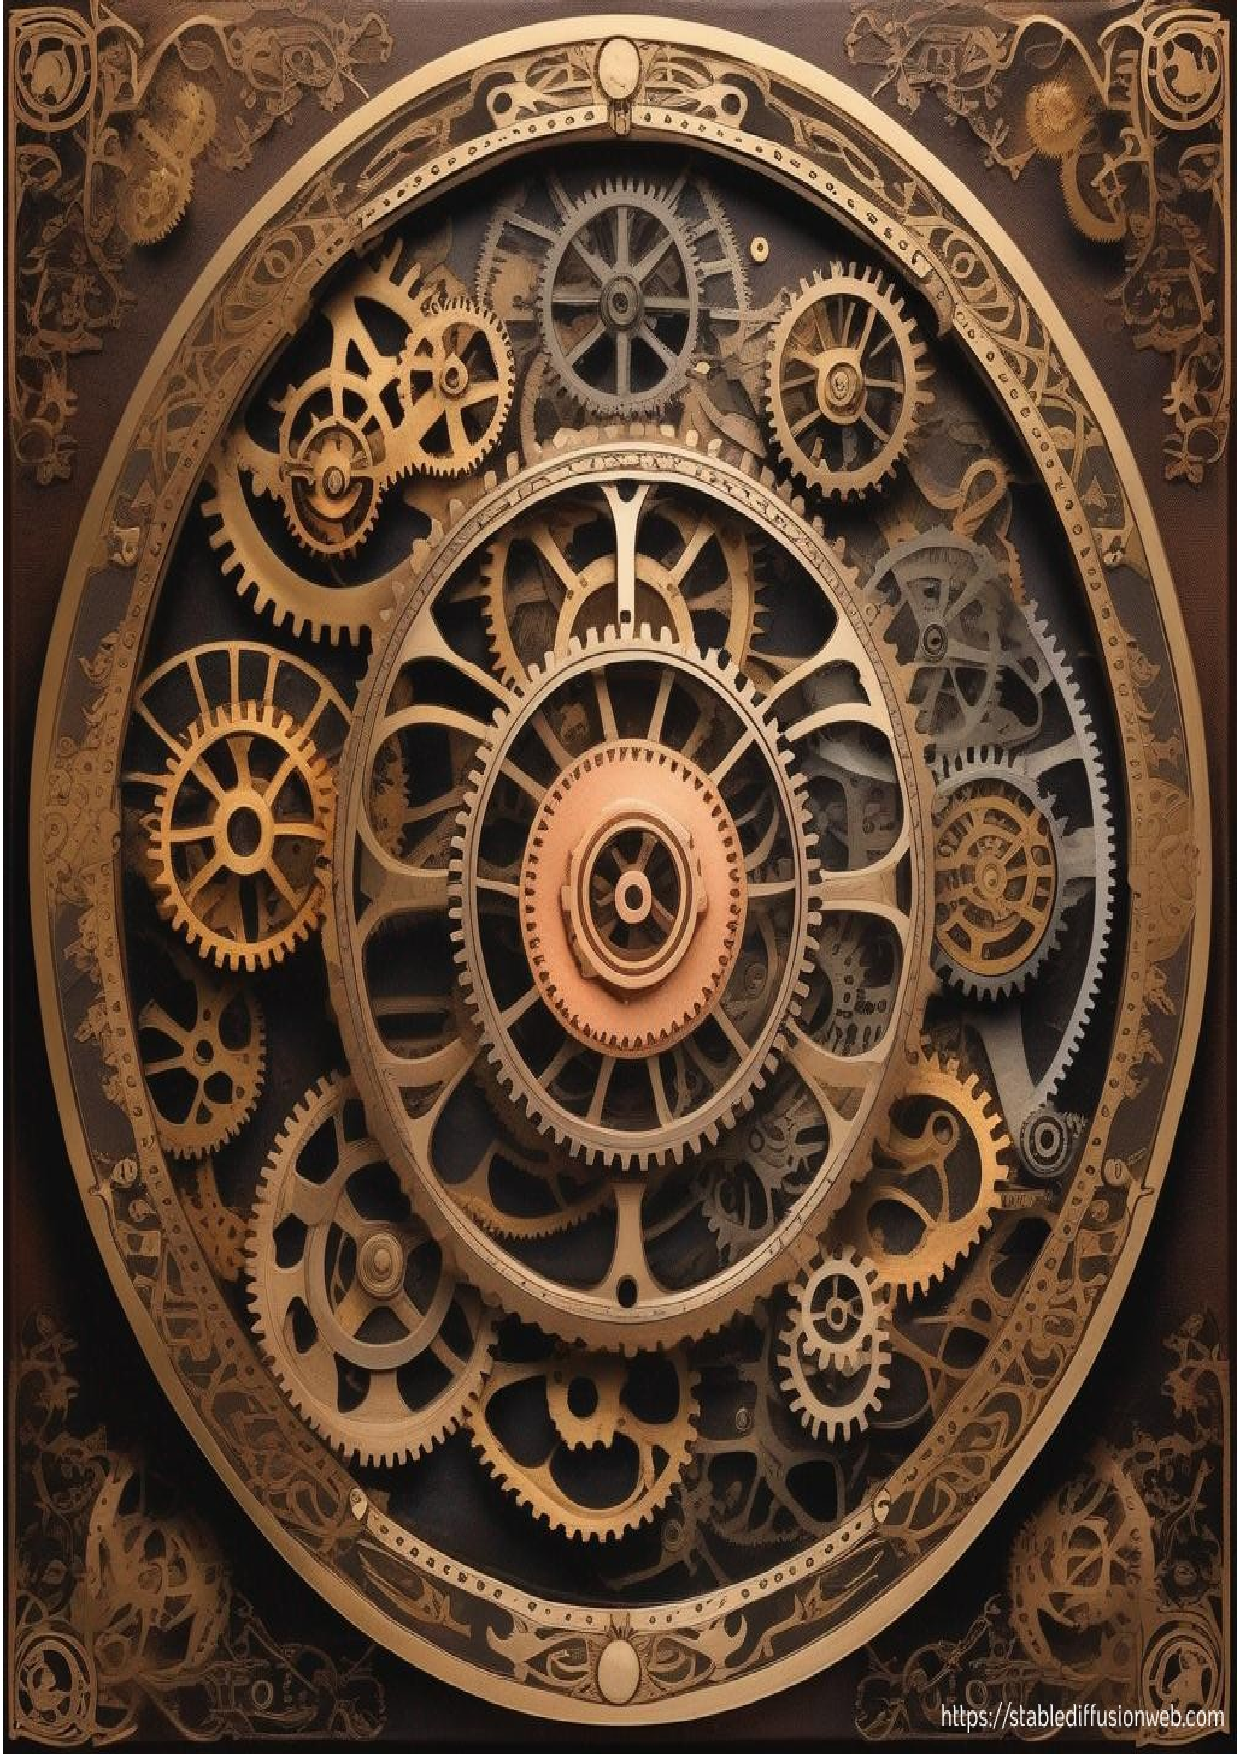
\includepdf{cover/backcover.pdf}

\end{document}
